\section{Aufbau und Durchführung}
\subsection{Aufbau}
\label{sec:Aufbau}

Zur Bestimmung der Wärmekapazität eines Materials, im vorliegenden Fall Kupfer, soll der Probe eine fest definierte Wärmemenge zugeführt werden.
Dazu wird der in Abbildung \ref{fig:aufbau} skizzierte Versuchsaufbau verwendet.

\begin{figure}
  \centering
  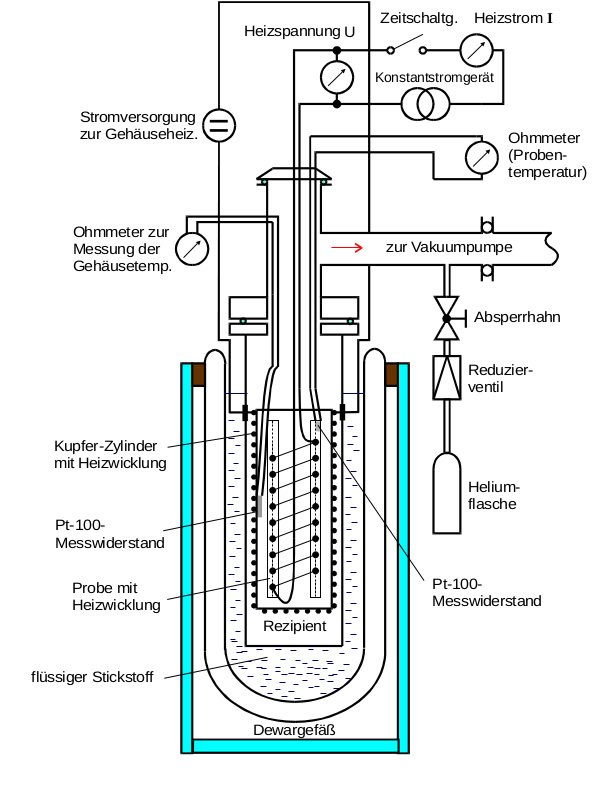
\includegraphics[height=13cm]{ressources/aufbau.png}
  \caption{Skizze zum Versuchsaufbau \cite{skript}.}
  \label{fig:aufbau}
\end{figure}

Um dem Kupfer die Wärme zuzuführen, ist der Körper mit einer Heizwicklung umgeben.
Dessen Stromzufuhr wird über ein Konstantstromgerät geregelt, die Heizspannung wird zusätzlich über ein Voltmeter abgelesen.
Die Probe befindet sich in einem Kupferzylinder, welcher ebenfalls über eine Heizwicklung mit einer eigenen Stromversorgung verfügt.
Hierdurch kann gewährleistet werden, dass der Zylinder während des Versuches die gleiche Temperatur wie das Probematerial besitzt, um einen Wärmeaustausch durch Konvektion oder Wärmeleitung zu vermeiden.
Der Kupferzylinder mit der Probe ist in einem Rezipienten, der mit einer Vakuumpumpe evakuiert werden kann.
Zusätzlich kann über ein Reduzierventil Gas, in diesem Fall Helium, aus einer Flasche in den Rezipienten geleitet werden.
Helium wird hier als Gas verwendet, da dieses ein deutlich besserer Wärmeleiter als Luft ist und die Abkühlung der Probe somit vereinfacht wird.
Der Druck im Rezipienten wird über ein Barometer gemessen.

Der gesamte Rezipient wird über eine Halterung in ein Dewargefäß gehalten.
Dieses Dewargefäß besitzt zwei Wände, in dessem Zwischenraum ein Vakuum vorhanden ist.
Dies unterstützt die thermische Isolierung des Versuchsaufbaus, da das Vakuum die Konvektion oder Wärmeleitung mit der Umgebung bestmöglich verhindert. %duh %corrected duuh
Zudem kann das Dewargefäß über einen Trichter mit flüssigem Stickstoff gefüllt werden, um die Probe zu kühlen.

Neben der festen Wärmezuführung muss auch die Temperatur, sowohl von der Probe als auch dem Kupferzylinder, gemessen werden.
Hierzu werden Ohmmeter, genauer Pt-100-Widerstände, als Widerstandsthermometer verwendet.
Diese Verwendung ist möglich, da der Widerstand von vielen Materialien, wie beispielsweise Platin, stark temperaturabhängig ist.
Die Umrechnung zwischen dem Widerstand und der Temperatur ist über eine monotone Funktion definiert, welche in der Auswertung angegeben wird.
